%!TEX root =../../../course-notes.tex
% ^ leave for LaTeXTools build functionality


\begin{applicationActivities}



\begin{observation}
Recall that we can model the velocity of a water droplet in a cloud by
\[mv'=-mg-bv\]
where here, negative denotes downward velocity.  \(m\) is the mass, \(g\) is Newton's gravitational constant, and \(b\) is a physical constant (like a coefficient of friction).
\begin{center}
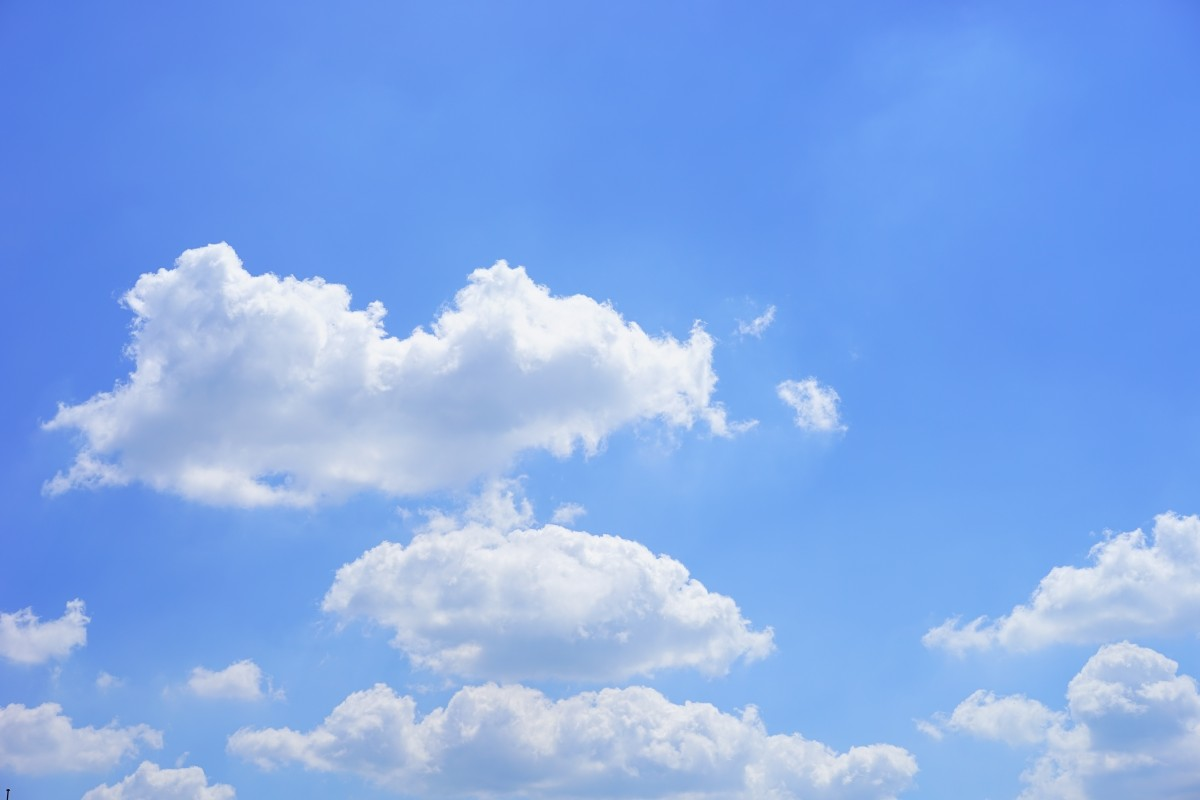
\includegraphics[scale=0.2]{media/cloud.jpg}
\end{center}
\end{observation}

\begin{activity}{25}
A water droplet with a radius of \(10\ {\rm \mu m}\) has a mass of about \(4 \times 10^{-15} {\rm kg}\).  It is determined in a laboratory that for a droplet this size, the constant \(b\) has a value of \(0.003 {\rm kg/s}\).
\begin{subactivity}
Write down the differential equation modelling this scenario.
\end{subactivity}
\begin{subactivity}
Find the general solution of this ODE.
\end{subactivity}
\begin{subactivity}
What is the terminal velocity of the droplet?
\end{subactivity}
\begin{subactivity}If the droplet starts from rest (\(v=0\)), what is its velocity after \(0.01\ {\rm s}\)?
\end{subactivity}
\end{activity}

\begin{definition}
The second part of the previous activity is an example of an \term{Initial Value Problem (IVP)}; we were given the initial value of the velocity in addition to our differential equation.
\end{definition}

\begin{activity}{10}
Solve the IVP
\[y'+3y=0, y(0)=2.\]
\end{activity}

\begin{activity}{10}
Solve the IVP
\[y'-2y=2, y(0)=1.\]
\end{activity}

\begin{activity}{5}
Solve the IVP
\[y'-2y=2, y(2)=1.\]
\end{activity}




\end{applicationActivities}
